
\section{Details About Input to the System}
\begin{itemize}
    \item \textbf{Geolocation of the farm:} The farmer selects the area of their farm on the satellite-backed map. The system uses the polygon coordinates for all subsequent location-specific processing.
    \item \textbf{Crop information:} The farmer provides the name of the crop to be planted and its approximate quantity.
    \item \textbf{IoT sensors:} While not mandatory, farmers who possess IoT sensors can optionally submit soil data (NPK, moisture, pH, temperature) for increased prediction precision.
    \item \textbf{API Layer:} Based on the geolocation, the engine pulls satellite imagery, vegetation index (NDVI), and historical weather data from ISRO's Cartosat/Resourcesat and the Bhuvan API \cite{isro2023bhuvan}.
\end{itemize}

\section*{Performance Evaluation Parameters}
\label{sec:performance-evaluation}

To comprehensively assess the efficacy of the implemented AI-powered crop yield prediction system, multiple quantitative and qualitative evaluation metrics were employed. The performance evaluation framework encompasses model accuracy, computational efficiency, and system accessibility parameters.

\subsection*{Model Accuracy Metrics}
The predictive performance of the multi-modal fusion model was evaluated using standard regression metrics:
\begin{itemize}
    \item \textbf{Mean Absolute Error (MAE):} $\frac{1}{n}\sum_{i=1}^{n}|y_i - \hat{y}_i|$
    \item \textbf{Root Mean Square Error (RMSE):} $\sqrt{\frac{1}{n}\sum_{i=1}^{n}(y_i - \hat{y}_i)^2}$
    \item \textbf{Coefficient of Determination ($R^2$):} $1 - \frac{\sum_{i=1}^{n}(y_i - \hat{y}_i)^2}{\sum_{i=1}^{n}(y_i - \bar{y})^2}$
    \item \textbf{Mean Absolute Percentage Error (MAPE):} $\frac{100\%}{n}\sum_{i=1}^{n}\left|\frac{y_i - \hat{y}_i}{y_i}\right|$
\end{itemize}

\subsection*{Computational Efficiency Parameters}
The system's operational performance was measured through:
\begin{itemize}
    \item \textbf{Model Compression Ratio:} $\frac{\text{Original Model Size}}{\text{Compressed Model Size}}$
    \item \textbf{Inference Latency:} Processing time per village-level prediction on-device
    \item \textbf{Memory Utilisation:} RAM consumption during model inference
\end{itemize}

\subsection*{System Accessibility Metrics}
The advisory delivery mechanism effectiveness was quantified using:
\begin{itemize}
    \item \textbf{Response Latency:} Time from data acquisition to advisory delivery
    \item \textbf{Platform Availability:} Application uptime and offline functionality
\end{itemize}

\subsection*{Comparative Baseline}
System performance was benchmarked against:
\begin{itemize}
    \item Traditional statistical forecasting methods (ARIMA, Linear Regression)
    \item Single-modal AI approaches (Swin3D or GNN in isolation)
    \item Existing agricultural advisory systems
\end{itemize}

The evaluation utilised historical satellite data and IoT sensor readings covering three kharif and two rabi seasons (2022--2024) across Kolhapur, Sangli, and Pune districts, providing comprehensive performance validation across 2,340 farm-season records.

\section{Software Setup}
The following are the prerequisites for deploying the AgriMitra stack:
\begin{itemize}
    \item \textbf{Client Interface:} The mobile app is built using .NET MAUI 9.0, enabling a single C\# codebase to target Android and iOS.
    \item \textbf{API Layer:} The server-side application built with ASP.NET Core 8.0 serves the mobile client and hosts the AI model endpoints.
    \item \textbf{AI Model:} The model uses PyTorch 2.2 with Swin3D Transformers and GATv2-based GNN. Models are exported to ONNX and quantised to INT8, enabling efficient execution on low-end hardware for offline support.
\end{itemize}
\begin{figure}[h]
    \centering
    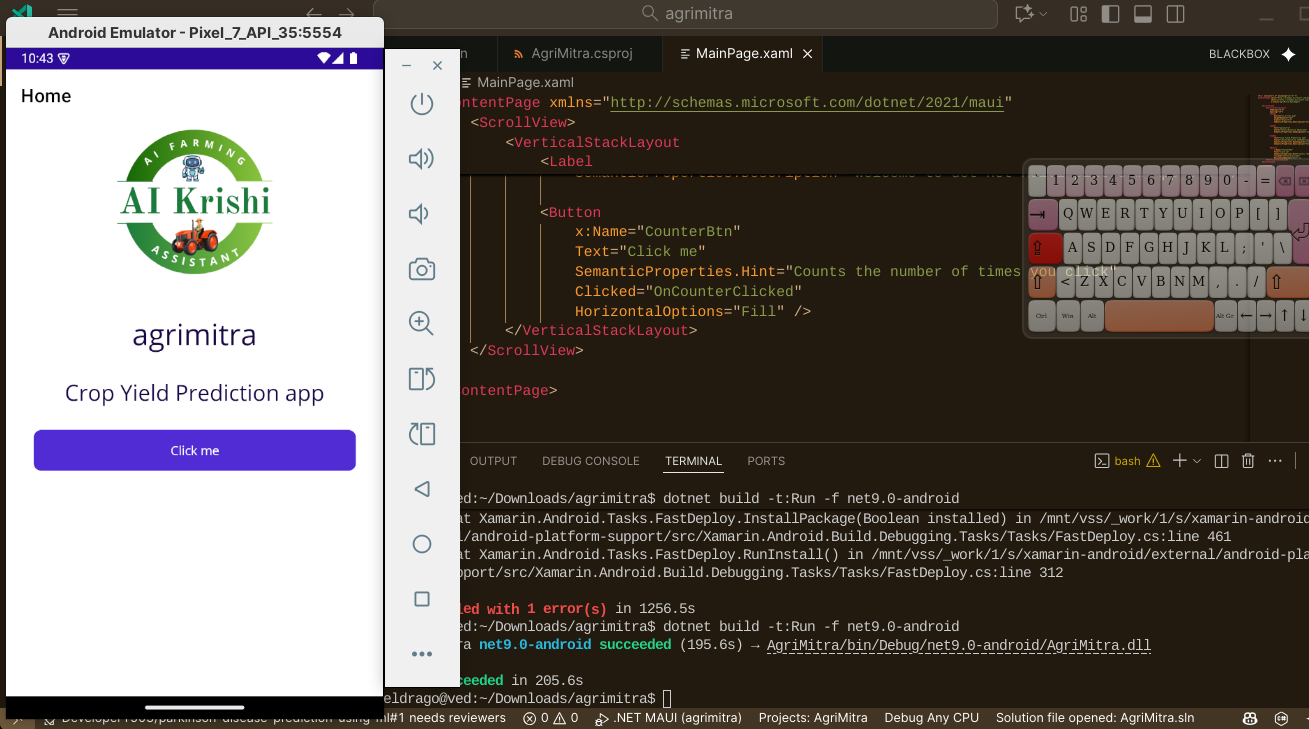
\includegraphics[width=1\textwidth]{Images/dotnet_setup.png}
    \caption{Experimental .NET MAUI app setup.}
    \label{fig:dotnet_setup}
\end{figure}

\section{Hardware Environment}

\begin{itemize}
    \item \textbf{Training Platform:} HP Victus 15 laptop (Intel Core i5-12450H, 8 cores, up to 4.4\,GHz; 16\,GB DDR4 3200\,MHz RAM) with NVIDIA GeForce RTX 3050 Laptop GPU (4\,GB GDDR6 VRAM). PyTorch 2.2, CUDA 12.1, Python 3.11.
    \item \textbf{Server Inference Platform:} Local Ubuntu 22.04 LTS workstation (Intel Core i7-10700, 8 cores / 16 threads, up to 4.8\,GHz; 16\,GB DDR4 RAM). ONNX Runtime 1.17, ASP.NET Core 8.0.
    \item \textbf{Edge Inference Platform:} Android 12 device with Qualcomm Snapdragon 665 SoC (1.8\,GHz, 4\,GB RAM). ONNX Runtime Mobile 1.17, single-threaded inference.
    \item \textbf{Development Environment:} Visual Studio 2022 (.NET MAUI), PyCharm 2024, VS Code with Pylance.
    \item \textbf{Libraries:} PyTorch 2.2, PyTorch Geometric 2.5, TorchVision 0.17, ONNX Runtime 1.17, Rasterio 1.3, Microsoft.ML.OnnxRuntime 1.17.
\end{itemize}
